\subsection{Economic factors: \textit{GDP growth}}\label{sec:quantification_economic}

\subsubsection{Definitions}

\begin{description}[style=nextline]
  \item[Gross Domestic Product (GDP) PPP]
        A measure of a country's economic output that accounts for differences in price levels between countries. By using PPPs and the common currency of international dollars, GDP PPP is adjusted for price level differences across countries, providing a more accurate measure of the economic output and living standards, as it reflects the real purchasing power of the citizens.

  \item[Purchasing Power Parity (PPP)]
        An economic theory that allows the comparison of the purchasing power of various world currencies to one another. It involves a comparison of the relative prices of a standard set of goods and services in different countries, thus providing a measure of the relative cost of living and enabling a more accurate comparison of economic well-being.
\end{description}

\boxparameter{GDP growth}{Slow stable growth}{Slow stable growth}{Slow stable growth}



\subsubsection{Sources of data}

The GPD projections for FutuRaM's future scenarios are based on economic data from the OECD as well as population data from Eurostat and the UK's ONS~\cite{oecd2021gdpdata,eurostat2023population,ons2023population}

\subsubsection{Results of projections}

As an `external element', the GDP projections do not differ across the scenarios, only as a function of time.

The results of the projections are shown in~\autoref{fig:gdp-projections}. An interactive figure can be viewed \href{https://futuram-project.github.io/FutuRaM.github.io/WP2/assets.html}{here~\faLink}

\begin{landscape}
\begin{figure}[h!]
    \centering
    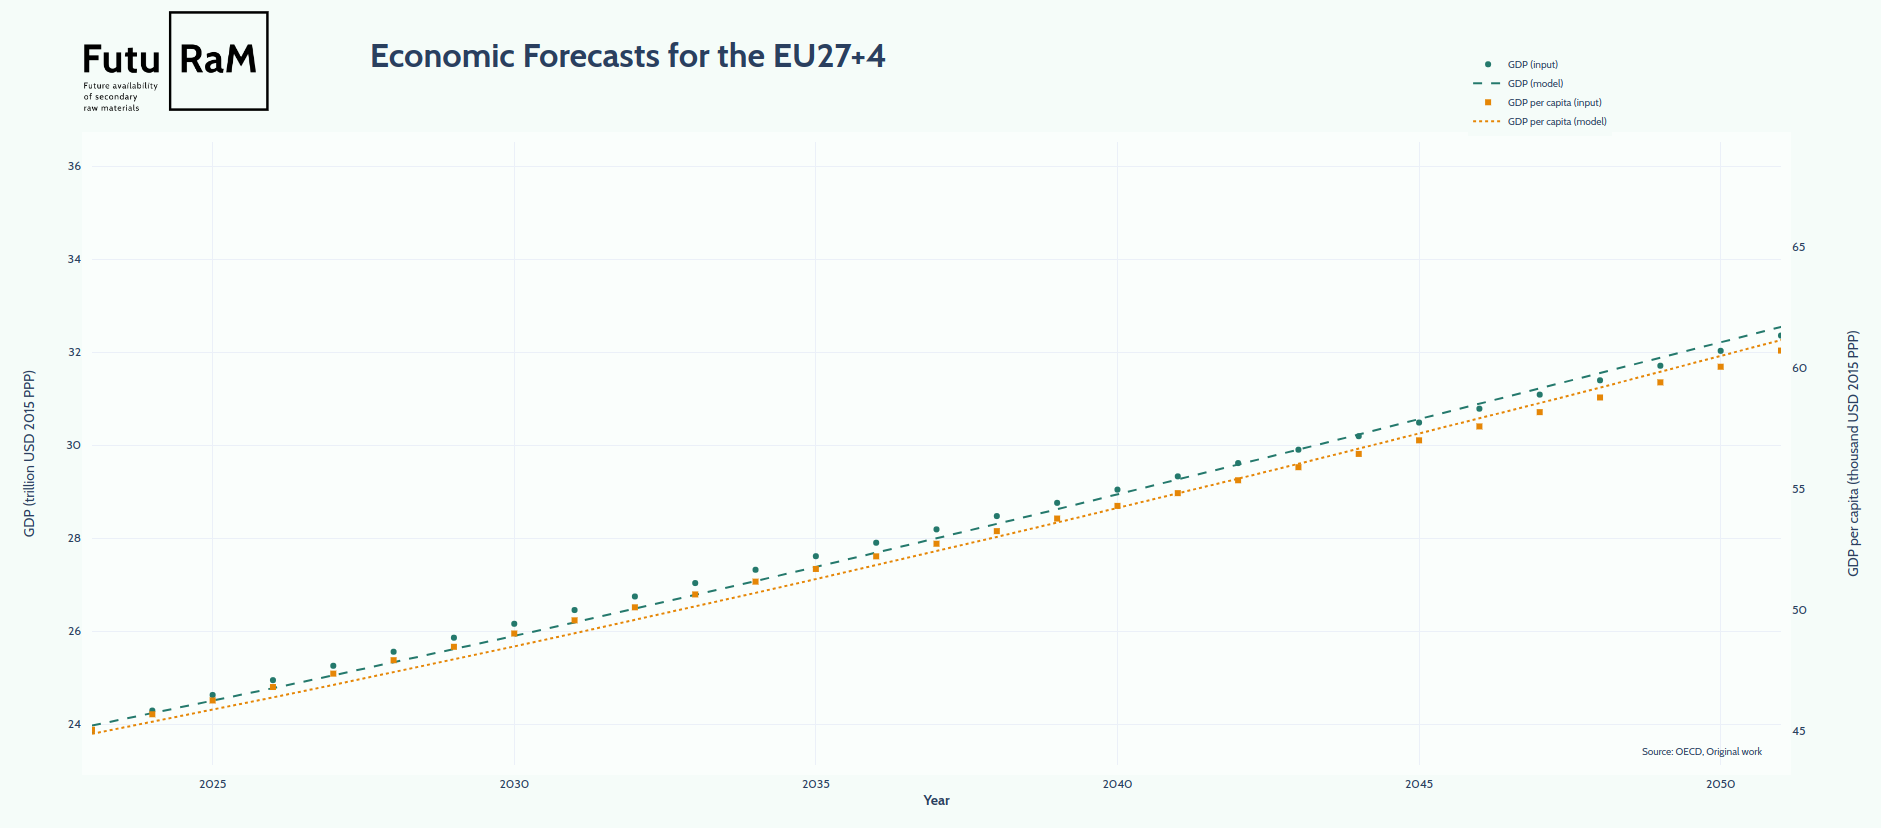
\includegraphics[width=\linewidth]{130quantification/external/gdp.png}
    \caption{GDP projections for the EU27+4}\label{fig:gdp-projections}
\end{figure}
\end{landscape}
\FloatBarrier

\subsubsection{Methodological Overview of OECD's GDP Projection Framework}~\cite{oecd2021gdpdata, oecd2021gdpmethod,duval2010gdp, oecd2012gdp}

The OECD's approach to projecting GDP is rooted in the principle that income levels across various nations will gravitate towards those observed in the most advanced economies, an idea put forth by~\cite{barro2004gdp, barro2004gdpbook}. This convergence is modelled through an enriched version of the Solow growth model, factoring in a dual-sector configuration~\cite{mankiw1992gdp}, which the OECD dubs the ENV-Growth model. Rather than focusing solely on convergence in income, the ENV-Growth model prioritises the growth factors that will drive GDP over time.

For GDP projections up to 2060, the OECD combines model-based assessments with expert evaluations, considering the economic dynamics of individual countries and the global market. These forecasts are denominated in the constant US dollars and PPPs of 2010, based on data from OECD and World Bank, which use the Atlas method for calculating PPPs~\cite{worldbank2023gdp,oecd2021gdpmethod}. The data originate from the OECD Long-Term Baseline Scenario. This scenario, which is integral to the OECD Economic Outlook, serves as a comparative standard to gauge the possible effects of structural reforms, assuming a policy-neutral environment. Conversely, long-term projections diverge from the medium-term forecasting model, which is predominantly demand-driven, by focusing on a supply-side perspective that takes into account labour and capital availability and productivity growth rates.



\subsubsection{Determinants of Long-term Growth}~\cite{fontagne2022gdp, oecd2021gdpmethod}


Recognizing the multifaceted nature of economic advancement, GDP growth projections consider an array of influences such as demographics, educational attainment, technological progress, energy access, and capital flow patterns. The MaGE framework facilitates GDP estimation by charting dynamic paths that reflect the structural interplay defining the economic landscape until 2050~\cite{fontagne2022gdp}.

The ENV-Growth model's projections span a century and include a wider selection of countries, enhancing the original methodologies developed by the OECD Economics Department~\cite{duval2010gdp, oecd2012gdp}. It introduces considerations for energy usage and resource revenue from oil and gas sectors, aligning with the enhanced sectoral approach for fossil fuels presented by~\cite{chateau2012gdp}.


The model's foundation lies in its projection of the five pivotal elements driving economic growth:

\begin{itemize}
  \item Physical capital
  \item Employment, shaped by population trends, age demographics, participation rates, and unemployment scenarios
  \item Human capital, based on education and its consequential effect on labour productivity
  \item Energy demand and resource extraction for exporting countries
  \item Total factor productivity (TFP)
\end{itemize}

The determinants of growth are not restricted to these factors; they also encompass a spectrum of social, economic, and institutional influences, including workforce education, trade openness, institutional integrity, fiscal strategies, regulatory frameworks, and demographic shifts. The underlying potential for economic catch-up through technology transfer and innovation is underscored by the differential in income between each country and the global technology frontrunner.

In the context of employment, projections from IIASA inform the total employment figures, combining time-specific participation rates for different age cohorts with projected unemployment trends. Education assumptions translate gender and age-specific educational projections into a human capital index, which then informs labour productivity enhancements.

For physical capital, the model follows a standard capital accumulation methodology with a set depreciation rate, with the investment rate per unit of GDP edging towards a balanced growth path level determined by the production function's structural parameters.

Energy and natural resources are integrated as productive components for consumers and as extra income from specific oil and gas sectors for producer nations. The model calibrates domestic energy productivity to historical improvement rates, progressing towards an efficiency frontier indicative of cutting-edge energy appliances. The economic contribution of energy resources to producer countries is extrapolated from resource depletion models that describe the dynamics between reserves and resources and the temporal evolution of marginal production costs.

FutuRaM's economic forecasts, while not based directly on the SSP data, are consistent with the SSP2 baseline derived from similar sources and models~\cite{ssp2017narrative, jiang2017ssp, leimbach2017ssp, cuaresma2017ssp, dellink2017ssp, samir2017ssp}, offering a comprehensive picture of potential economic trajectories.


\begin{figure}[h!]
  \centering
  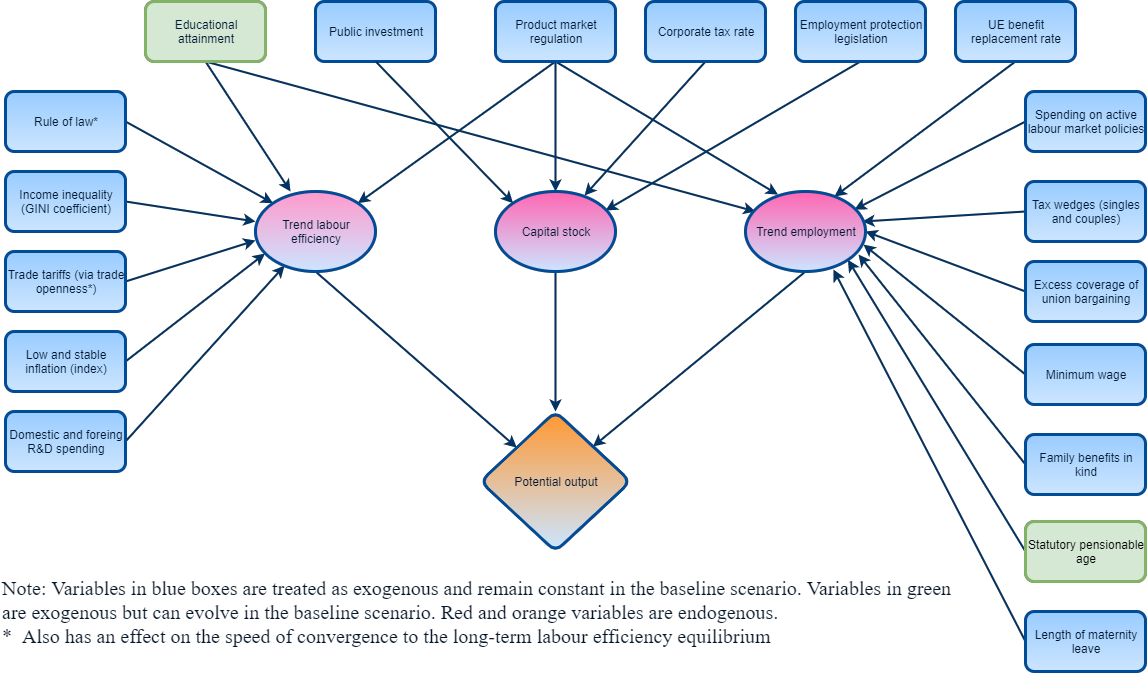
\includegraphics[width=\textwidth]{130quantification/external/oecd2021gdpmethod_drivers.png}
  \caption[Factors incorporated in the long-term GDP model]{Factors incorporated in the long-term GDP model~\cite{oecd2021gdpmethod}}\label{fig:gpd_method}
\end{figure}

\clearpage
\subsubsection{Implications of GDP Growth on FutuRaM's Waste Models}

GDP growth has significant implications for models concerning secondary raw material recovery and waste generation. For example, increasing GDP tends to lead to higher consumption levels, which can result in more waste generation across various streams. However, higher income also provides greater resources for investment in recovery technologies and infrastructure. Below are some examples for each of the specified waste streams.

\wasteSubsubsubsecBATT

As GDP grows, the demand for electronic devices and electric vehicles typically increases, leading to a higher turnover of batteries. This could necessitate advancements in recovery methods for battery components, such as lithium and cobalt, to reduce reliance on primary sources and mitigate environmental impact.

\wasteSubsubsubsecCDW

Economic growth often spurs construction activity, thereby increasing CDW. Increasing GDP as a ratio of waste generation could lead to enhanced recycling processes, promoting the circular economy by converting waste into secondary raw materials for new construction projects.

\wasteSubsubsubsecELV

The number of ELVs rises with economic prosperity, as people can afford newer vehicles more often. This creates opportunities to recover valuable materials and components, necessitating more efficient recycling processes.

\wasteSubsubsubsecMIN

As economies expand, so does the demand for minerals, potentially increasing mining waste. With increased GDP, there could be more investment in techniques to minimise waste generation and recover valuable materials from mining by-products.

\wasteSubsubsubsecSLASH

Higher GDP can correlate with increased industrial activity, producing more slags and ashes. Enhanced recovery techniques can transform these by-products into useful secondary raw materials, such as aggregates in construction.

\wasteSubsubsubsecWEEE

GDP growth can lead to shorter replacement cycles for electronic goods, increasing the amount of WEEE. There's a potential for improved recovery of precious metals and rare earth elements, driving innovation in e-waste recycling technologies.

\clearpage

\subsubsection{Incorporation of economic growth into individual waste stream models}

\boxws{This section will be filled out with the details of exactly how this parameter is incorporated into your stock and flow models}

\wasteSubsubsubsecBATT
\begin{itemize}
    \item X
\end{itemize}

\wasteSubsubsubsecCDW
\begin{itemize}
    \item X
\end{itemize}

\wasteSubsubsubsecELV
\begin{itemize}
    \item X
\end{itemize}

\wasteSubsubsubsecMIN
\begin{itemize}
    \item X
\end{itemize}

\wasteSubsubsubsecSLASH
\begin{itemize}
    \item X
\end{itemize}

\wasteSubsubsubsecWEEE
\begin{itemize}
    \item X
\end{itemize}



\subsubsection{Conclusion}

Economic growth can therefore act as both a driver of waste generation and a catalyst for innovation in the recovery of secondary raw materials. The challenge for models like FutuRaM lies in accurately predicting these trends and proposing effective strategies to balance economic benefits with environmental sustainability.

\boxreview{This conclusion will be more completely compiled once the individual waste stream sections for each parameter are complete.}

\sectionEndlines

\clearpage

